\documentclass[a4paper]{article}

%% Language and font encodings
\usepackage[english]{babel}
\usepackage[utf8x]{inputenc}
\usepackage[T1]{fontenc}

%% Sets page size and margins
\usepackage[a4paper,top=3cm,bottom=2cm,left=3cm,right=3cm,marginparwidth=1.75cm]{geometry}

%% Useful packages
\usepackage{amsmath}
\usepackage{graphicx}
\usepackage[colorinlistoftodos]{todonotes}
\usepackage[colorlinks=true, allcolors=blue]{hyperref}

\title{Brazilian/British Music Variations during the week}
\author{Arthur Costa}

\begin{document}
\maketitle

\begin{abstract}
This paper is intended as a project for the discipline of Data Science in the UFPE. There are no scientific purposes on this article, however there will be used some methods to confirm the observations, and hopefully it will generate some fun trivia.
\end{abstract}

\section{Obtaining Data}

To obtain data about music trends in these countries, with a more in depth data than the most basic ones, I had to choose a platform that would allow me to get this data somehow. The one I chose was LastFM, to crawl users, and get the musical history from each one. To get more data about each music I chose to query Spotify API as they had more data on tracks.

\subsection{Finding users on LastFM}

To start, the initial thing was getting a few users as seed, and then for each user query its friends. There were 3 queues for users, 1 for brazilians, 1 for Uk users, and 1 for other users. On each round, one user was taken from one of the queues(brazilian one first, if it was empty or had 10 more brazilians processed then would choose Uk one, and would only get from the 3rd one if there was no one from br or uk), would see 100 of his friends, and query his nationalities, and put on each queue according to each nationality(if it wasn't processed before).

\subsection{Getting musical history from each user on LastFM}

When each user is taken from the queue, if he is from Brazil or UK the crawler will query LastFM for it's last 1000 musics. Then this musics are queried on Spotify to get their features.

\subsection{Getting music features info about the musics from Spotify}

Each music was searched by the name on Spotify, that gives a little of noise on musics with same name, but not enough to show into calculations. The Features extracted were 9: acousticness, danceability, energy, instrumentalness, liveness, loudness, speechiness, tempo, valence.

\subsection{Aggregating musical features by time in the week and country}

As it was known the country of each user, it was needed to put all data from each country summed up aggregated by hour of week.

\subsection{Statistics about the data crawled}

200 hundred users were processed, being roughly 90 from each country. 76061 Songs from brazilian users, and 66295 from UK users. Over 150k requests were made during this data gathering.

\section{Data Observations}

\subsection{Overall comparisons}

Getting a comparison per category, on which tops which to then get some conclusions about the feature averages over each country.
\begin{table}
\centering
\begin{tabular}{l|c|r}
Feature & Brazil & United Kingdom \\\hline
Acousticness & 0.3070522150555476 & 0.314761650420092 \\
Danceabilty & 0.5181635910650663 & 0.5409404253714458 \\
Energy & 0.6183142958835671 & 0.6010829950991778 \\
Instrumentalness & 0.1632221673711889 & 0.20346305205068257 \\
Liveness & 0.20991806655184653 & 0.1985800980466098 \\
Loudness & -9.042842889259939 & -9.250683792141187 \\
Speechiness & 0.07570553108689079 & 0.08827292254317823 \\
Tempo & 120.14557384204781 & 118.99128139377027 \\
Valence & 0.4547096533045844 & 0.4479696824798251

\end{tabular}
\end{table}

\subsubsection{Observations on the averages}

Brazil and United Kingdom are very close on almost all averages however a few things were strange, and here are they:

\begin{enumerate}
\item The instrulmentalness was close to 25\% bigger on the UK, what might imply that brazilian musics are more about singing, or since the measure of instrumentalness is a probability the only thing that can be that both countries are not very into instrumental music.
\item Loudness is 0.20 less in the UK than in BR, and remember that loudness is based on logarithm so UK music is 20\% calmer than the musics that brazilians listen to.
\item Danceability is bigger in the UK by 5\%, what is against my initial conceptions before this study.
\end{enumerate}
\subsection{Exploring hours of the day}
Here there will be graphs showing the data, and will use the dashed green lines to represent brazil, and the continuous blue line for the UK.
\subsubsection{Tempo over the day}
\begin{figure}[h]
\centering
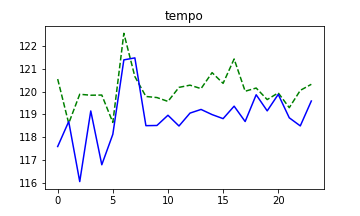
\includegraphics[width=200px]{tempo_daily.png}
\end{figure}
Brazil songs stay 2 beats per minute above the UK almost all the day, there is a strange spike in the morning where might be caused by people trying to start the day more agitated. 

\newpage
\subsubsection{Count over the day}
\begin{figure}[h]
\centering
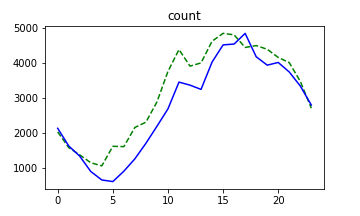
\includegraphics[width=200px]{count_daily.png}
\end{figure}
Although both countries seem similar on the count along the day, the fact that we can see the number of musics increasing by 5x from 5 AM to 5 PM, still is impressive. Caused by the sleep time, no doubt, however knowing the hours music is listened to is useful on ads targeting.

\subsubsection{Loudness and Energy over the day}
\begin{figure}[h]
\centering
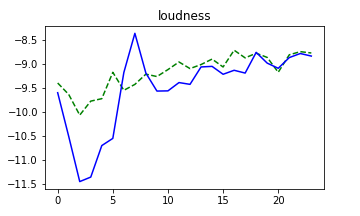
\includegraphics[width=200px]{loudness_daily.png}
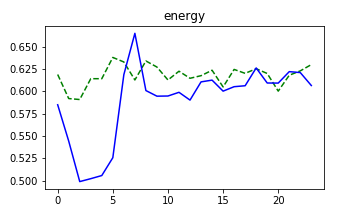
\includegraphics[width=200px]{energy_daily.png}
\end{figure}
There is a clear correlation(plotting actual correlation got me 0.923330) between uk loudness and energy, what might be as one of the parameters to calculate energy might be the loudness.

There is a drop on the energy and loudness between 2 AM and 5 AM in the UK, what might suggest that people from the UK prefer calmer songs during the night period.

\subsubsection{Acousticness over the day}
\begin{figure}[h]
\centering
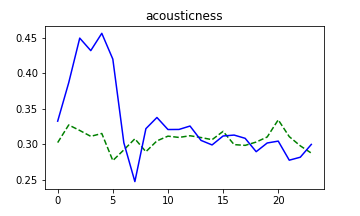
\includegraphics[width=200px]{acousticness_daily.png}
\end{figure}
There is a rise on the acousticness on the same time the loudness/energy goes down. So led to the thought that the correlation is inverted, and what was found by calculating correlation confirmed the idea, there was a -0.966364  energy-acousticness correlation. That might be caused as acoustic songs tend to be way calmer.
\newpage
\subsection{Exploring days of the week}
The week graphs were made in a way that Monday is the day 0, and 6 is Sunday. 
\subsubsection{Loudness over days}
\begin{figure}[h]
\centering
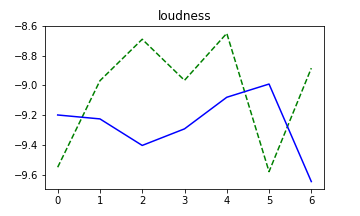
\includegraphics[width=200px]{loudness_weekly.png}
\end{figure}
While music in the UK gets louder closer to the weekends, while brazilians get calmer on the saturdays.
\subsubsection{Count over days}
\begin{figure}[h]
\centering
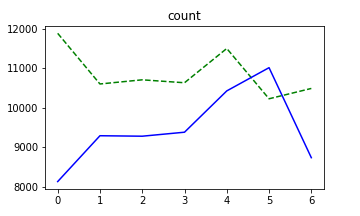
\includegraphics[width=200px]{count_weekly.png}
\end{figure}
Finally the count during the week, while brazil goes down along the week, and UK goes up as weeks passes by, while there is a clear pattern on the UK one. UK pattern is aligned with the expectations that people listen more closer to weekends, where they will go out. However there is no clear pattern on the brazil count.
\section{Problems}
Here I will point the mistakes done in this article, as again it was not meant to be used into other scientific purposes, and is actually meant to learn on data analysis, I decided to point out mistakes done during this study.
\subsection{Gathering data}
\subsubsection{Handling errors}
The APIs were failing on some of the calls, and the error handling was not perfect so there were some losses on a few of the users. 
\subsubsection{Granularity}
I assumed I didn't need a bigger granularity than the hour so I didn't get more granular than that on collecting data, that should be done on the processing, not on getting data, as I would want use more granular data later.
\subsubsection{Raw Data}
I didn't save the raw data, and if I had saved the whole raw data I would not have the problem 3.1.2, and would be able to test things using p tests.
\subsubsection{Taking care of timezones}
When I collected the data it was not considering timezones, so I had to take that into account later.
\subsection{Analyzing Data}
\subsubsection{Colors only graph(fixed later)}
During the creation I chose color based graphs, so I realized the mistake that it would be awful for color blind people, and fixed it.
\subsubsection{Count Normalization}
The raw count wasn't the best option to visualize frequencies as there was 10k more from brazil. I should have normalized it.
\subsubsection{Treating data in wrong formats}
The fact that instrumentalness was a probabilty was not well taken into account during some parts, as it didn't make much sense to use an average for it.
\end{document}